\subsection{Парабола}
\begin{wrapfigure}[11]{l}{0.5\tw}
	\centering
	\vspace{-.7pc}
	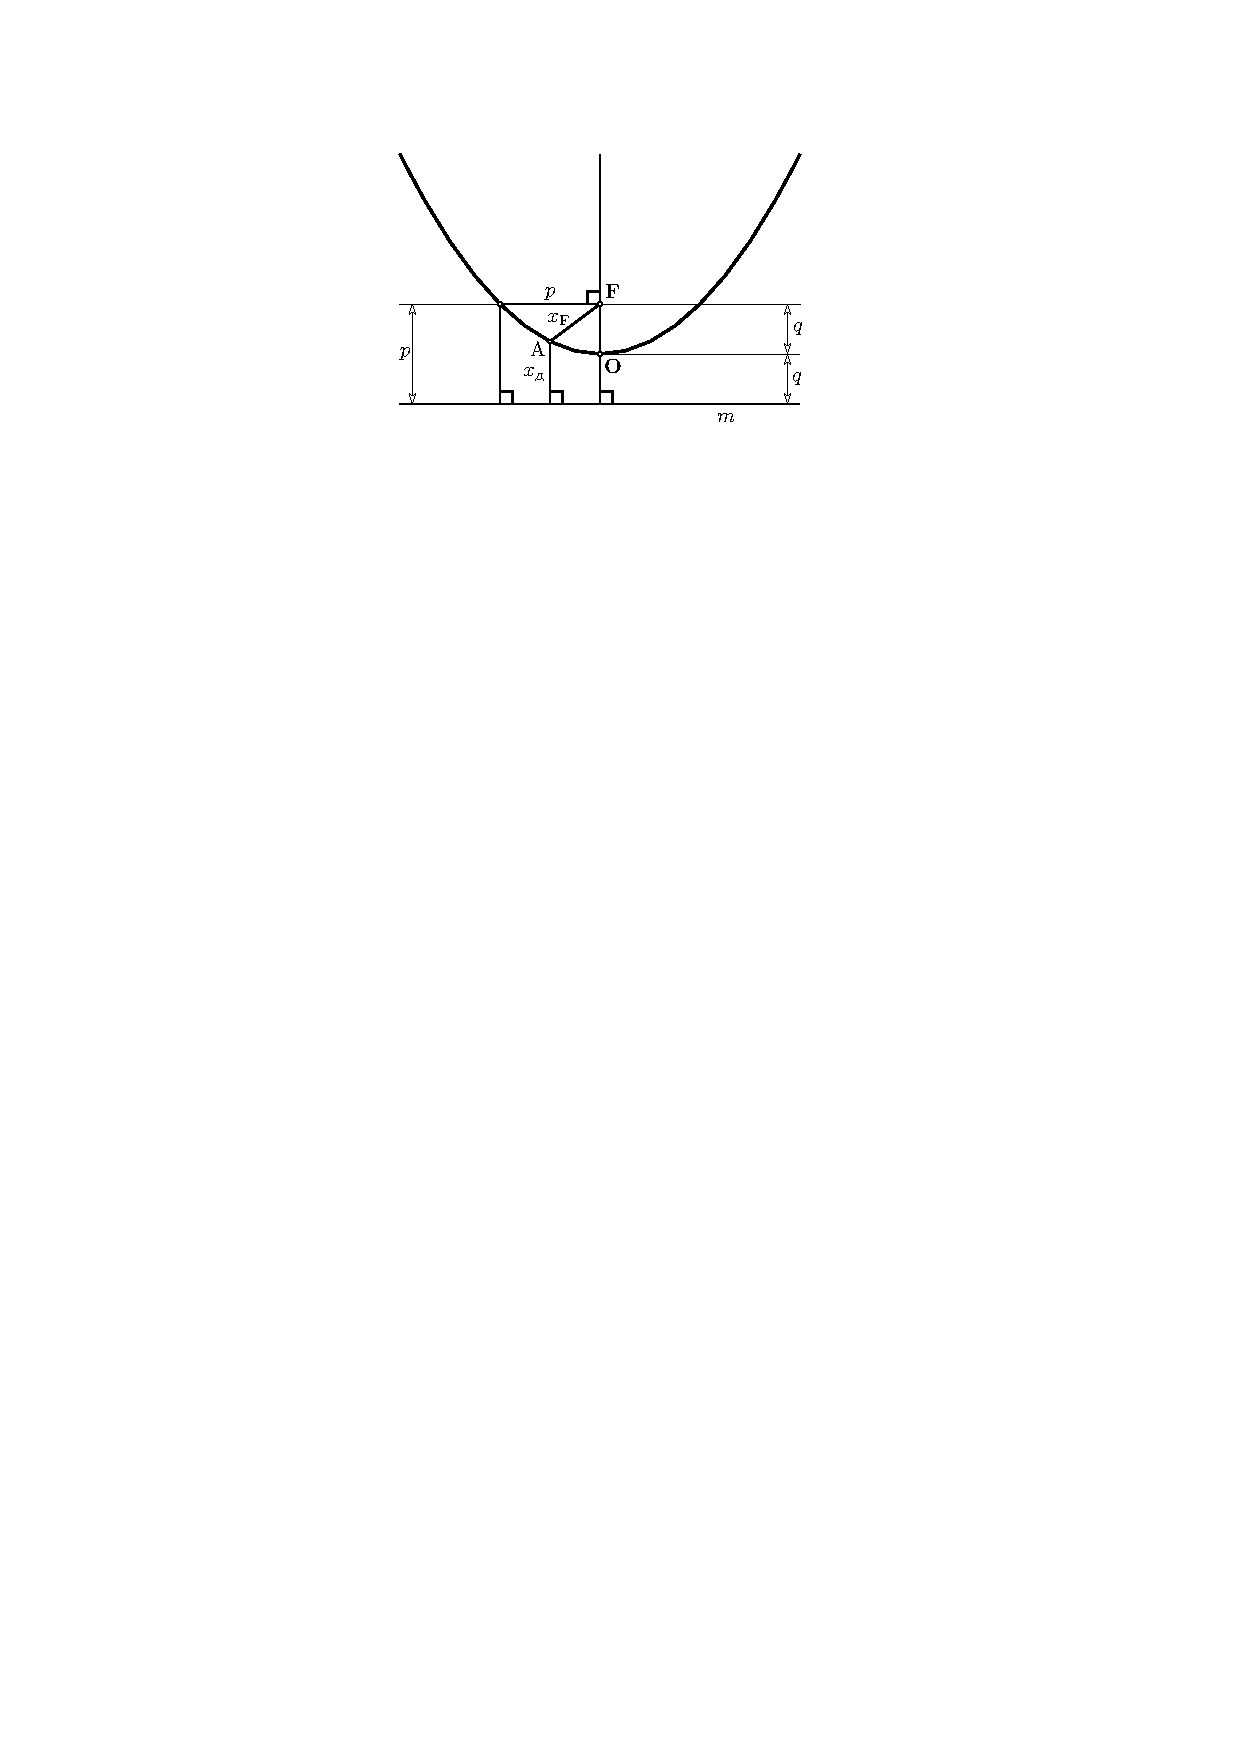
\includegraphics[width = 0.5\tw]{Parabola}
	\captionof{figure}{Парабола \label{pic:the-pic}}
\end{wrapfigure}
{\bfseries \term{Парабола}} --- геометрическое место точек, равноудалённых от данной прямой (называемой \term{директрисой} параболы) и данной точки (называемой \term{фокусом} параболы).

{\itshape Каноническое уравнение параболы}:
\begin{equation}
	y^2=2px,
\end{equation}
где $p$~--- \term{фокальный параметр}, равный расстоянию между фокусом параболы и директрисой или удвоенному расстоянию между фокусом параболы и вершиной.

Парабола в полярной системе координат $(r,\varphi)$ с центром в фокусе и нулевым направлением вдоль оси параболы (от фокуса к вершине) может быть представлена в виде уравнения
\begin{equation}
	r = \frac{p}{1 + \cos\varphi}.
\end{equation}
Эксцентриситет параболы равен $e=1$. Важно отметить, что парабола не имеет \term{большой} и \term{малой полуоси}.

Как и все конические сечения, парабола обладает \textit{оптическим свойством}, которое формулируется следующим образом: пучок лучей, параллельных оси параболы, отражаясь в параболе, собирается в её фокусе. И наоборот, свет от источника, находящегося в фокусе, отражается параболой в пучок параллельных её оси лучей.
